% !TeX encoding = UTF-8
% !TeX program = pdflatex
% !BIB program = biber

%%% To write an article in English, please use the option ``english'' in order
%%% to get the correct hyphenation patterns and terms.
%%% \documentclass[english]{class}
%%% for anonymizing an article you can use the ``anonymous'' option.
%%%
%%% Um einen Artikel auf deutsch zu schreiben, genügt es die Klasse ohne
%%% Parameter zu laden.
%%% Zur Anonymisierung kann die ``anonymous'' Option genutzt werden.
\documentclass[english]{lni}
\usepackage{dirtytalk}
\usepackage{graphicx}

\addbibresource{sources.bib} 


%%
\begin{document}
%%% Mehrere Autoren werden durch \and voneinander getrennt.
%%% Die Fußnote enthält die Adresse sowie eine E-Mail-Adresse.
%%% Das optionale Argument (sofern angegeben) wird für die Kopfzeile verwendet.
\title[Ein Kurztitel]{Exposé for the Master's Thesis \textit{Augmenting Enterprise Architecture Landscapes with AI: A Retrieval-Augmented Chatbot Approach using Graph Databases}}
%% \subtitle{Untertitel / Subtitle} % if needed
 \author[1]{Hendrik Gruber}{hendrik.gruebr@stud.fra-uas.de}{}
 \affil[1]{Frankfurt Univeristy of Applied Sciences}
\maketitle

%\begin{abstract}
%Dies ist eine kurze Übersicht über das Dokument mit einer Länge von
%70 bis 150 Wörtern. Es sollte ein Absatz sein, der die relevantesten
%Aspekte enthält.
%\end{abstract}


This exposé outlines what, why, and how the work for my planned master's thesis will be conducted. The goal of this exposé is to provide an overview of the subject matter and to demonstrate my understanding of the research topic.

\begin{keywords}
AI chatbot, Retrieval-Augmented Generation (RAG), Enterprise Architecture Management (EAM).
\end{keywords}
%%% Beginn des Artikeltexts
%\section{Überschrift/Heading}


\section{Problem Statement and Research Questions}
Within the realm of Enterprise Architecture Management (EAM), updating and maintaining the architecture landscape and documentation when new projects or applications arise can be a tedious task. It requires that the Enterprise Architect (EA) understands the landscape of existing projects and applications and the changes required to reflect these new incoming initiatives in a way that preserves consistency, avoids redundancies in the landscape, and supports the organization's strategic goals. Because the landscape of a company can be highly complex, containing hundreds of applications and projects, seeing the big picture can be a difficult task for an individual or even for an entire team. \textbf{todo Quelle}

This is a laborious task which can potentially be supplemented with the help of generative AI \textbf{todo Quelle}. AI can read in application landscape diagrams and project descriptions written in natural language and embed it into a graph database allowing an EA to retrieve information via chat. However, as it stands, there is a lack of GenAI solutions for this specific problem. All publicly existing solutions either have outdated models or are only theoretical work.

The master's thesis will be tackling the following research question: \say{\textbf{How can generative AI support Enterprise Architects in assessing and documenting the effects of new or changing projects on the application landscape?}} Three supplementary questions will be answered when approaching the main thesis questions:
\begin{enumerate}
    \item \say{What are the current challenges faced by Enterprise Architects when updating landscapes and documenting changes when new projects occurr?}
    \item \say{How can application and project descriptions be transformed into graph-based representations that integrate with existing landscapes?}
    \item \say{How effective is a generative AI chatbot in supporting Enterprise Architects compared to traditional EAM tools?}
\end{enumerate}


\section{Literature and State of the Art}
The following literature research was conducted as a preliminary search in order to understand what gap my thesis can fill. Google Scholar was primarily used and academic sources after 2022 were predominantly used, especially for sources regarding chatbots and AI. ChatGPT's deep research feature was also used as a supplement research method after describing to it what my thesis subject is about. This list of literature is not exhaustive and further research will be conducted for the final thesis. The sources are clustered and briefly described as follows.

\subsection{Enterprise Architecture Management}
The book from 2021 by \cite{jung2021masterclass} goes into detail on how EAM works, what challenges EAs face during their tasks, and gives a foundation to build upon when analyzing how to improve the process of documenting changes. Especially chapter 5 will give a scientific basis for everything regarding EAM and EAs.

\subsection{Human-Chatbot-Interaction}
The 2025 paper from \cite{ramachandran2025transforming} focuses on how software architects can leverage chatbots such as ChatGPT to aid in creating software diagrams such as UML diagrams. The paper notes limitations when creating actual diagrams. They were often inconsistent and less robust than the human-created version. Some chatbots were also very sensitive to the input prompts. This is relevant for my thesis as the EAM chatbot will also be generating some sort of output and knowing what to be cautious of beforehand will aid in improving the output.

\subsection{Graph Databases and Graph Embeddings}
The 2023 paper from \cite{besta2023demystifying} gives a solid foundation on how graph databases work. It covers how they organize data, how they are designed, and what types of queries a graph database can support. This paper will deem useful to understand and describe the basic functionality of graph databases.

Taking complex data such as the landscape diagrams and project descriptions and embedding it in a graph database in a way that represents the data correctly will be one of the main challenges during the implementation phase. The 2020 paper from \cite{grohe2020word2vec} describes that the quality of the vector representations is decisive is for usefulness of the data. This paper gives an overview of different embedding methods such as word2vec and methods to understand the embeddings.

\subsection{Large Language Models and Retrieval-Augmented Generation}
The 2024 paper by \cite{zhao2024retrieval} describes how RAG works and how it supplements LLMs in order to allow domain-specific answers. It also describes the challenges of retrieving the augmented data, accurately interpreting the user's intent, and fully harnessing the capabilities of the LLM. This paper will serve as a solid foundation on which my thesis can build.

What stands out is that there is no practical implementation of an RAG-based AI chatbot which helps EAs with their workload when documenting a changing landscape. This is the literary gap that my thesis will attempt to fill.

\section{Methodology and Approach}
Conducting this research will require a prototype-driven approach. An AI chatbot will be developed with which an EA can interact. The chatbot will be trained with real-world data and will be able to augment generated responses by accessing this data in a graph database. The EA will be able to use natural language within a chat prompt, similar to the UI of existing chatbots such as ChatGPT. It will be able to hold a conversation with the EA about the planned changes and effects.

\subsection{System Architecture}
The architecture of the prototype will consist of five basic elements, as shown in figure \ref{fig:arch_diagram}. The provided data, which contains project and application factsheets, will be vectorized and read into a graph database. The advantage of a graph database in this case is that similar projects will be represented by similar vectors \textbf{todo mit quelle}. Once the data is stored in the database, the LLM is able to retrieve data from the database and augment its response with the real-world project data. An out-of-the-box LLM will be used in this case and no new LLM will be trained.

The EA will then be granted access to a web application containing a chat UI. The EA may ask questions such as "For project x, I need to be able to document requirements and manage progress on tasks. I need new software for this and need to understand how my application landscape will by affected by this and how to document it." The chatbot will be able to ask for more information and get everything it needs from the EA to be able to answer the question. It then makes a suggestion on what the EA can do and and updates the documentation and landscape accordingly. The LLM will be prompted to stick to the topic of EAM and is able to hold a conversation on the subject matter.

\subsection{Anticipated Challenges}
Implementing this prototype will come with its own challenges as contains complex requirements. One foreseeable challenge will be converting the provided data into vectors, nodes, and edges and inserting it into the graph database in such a way that the data can later be augmented in realtime. Many different methods exist to embed data into vectors, nodes, and edges and finding a method that represents the project and application landscape in a useful way is a hurdle that needs to be overcome.\cite{grohe2020word2vec}

Another challenge may be heterogeneous data formats or generally inconsistent data. The format of the factsheets may be different or have different data types. Some project's or application's factsheets may also have varying depths of information. E.g. one project may be described in detail while another project may only be described at surface level.

The effects of data complexity and the corresponding risk of latency is currently not known. If there are hundreds of application and project descriptions which will be embedded into the vector database, then applying RAG on large scale graph database could potentially cause latency in response times. The actual impact of this will have to be kept in mind.


\begin{figure}[h]
\centering
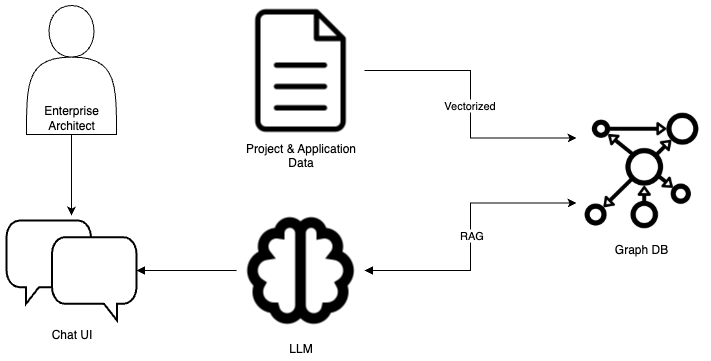
\includegraphics[scale=0.5]{./architecture_diagram.png}
\caption{A first draft architecture diagram of the expected system components and points of interaction between them.}
\label{fig:arch_diagram}
\end{figure}

\section{Expected Contribution}
The contribution of this thesis is to propose a scientifically sound methodology for building an LLM-based chatbot in the realm of EAM. The work will identify strengths and limitations of combining graph-based knowledge with retrieval-augmented generation, and will derive design principles and evaluation criteria for such systems. Furthermore, the thesis will provide guidance on how to critically assess embedding quality, retrieval effectiveness, and the trade-offs involved in integrating structured and unstructured data. In doing so, it contributes both practical insights for enterprise architects and a foundation for future research on AI-assisted EAM tools.

\section{Thesis Outline and Structure}
The following general structure will be followed for the thesis:

\begin{itemize}
    \item Introduction, Motivation, and Thesis Question
    \item Background Information (Foundational Concepts such as EAM, LLMs, RAG, Graph DBs)
    \item Current State of the Art and Literature
    \item Methodology and System Design
    \item Evaluation setup (metrics, test data), Evaluation of Results, Discussion of Findings, and Challenges \& Limitations
    \item Conclusion and Future Work
\end{itemize}




\printbibliography
\end{document}
